% CS615A Aspects of System Administration
% Author: Jan Schaumann <jschauma@netmeister.org>
% $Id: slides.tex,v 1.12 2006/02/12 23:15:03 jschauma Exp $

\special{! TeXDict begin /landplus90{true}store end }

\documentclass[xga]{xdvislides}
\usepackage[landscape]{geometry}
\usepackage{graphics}
\usepackage{graphicx}
\usepackage{colordvi}
\usepackage{tabularx}
\usepackage{multirow}

\begin{document}
\setfontphv

%%% Headers and footers
\lhead{\slidetitle}                               % default:\lhead{\slidetitle}
\chead{CS615 - Aspects of System Administration}% default:\chead{\relax}
\rhead{Slide \thepage}                       % default:\rhead{\sectiontitle}
\lfoot{\Gray{Multiuser Fundamentals, Ethics, Automation I}}% default:\lfoot{\slideauthor}
\cfoot{\relax}                               % default:\cfoot{\relax}
\rfoot{\Gray{\today}}

\vspace*{\fill}
\begin{center}
	\Hugesize
		CS615 - Aspects of System Administration\\ [1em]
		Multiuser Fundamentals, Ethics; Automation I\\ [1em]
	\hspace*{5mm}\blueline\\ [1em]
	\Normalsize
		Department of Computer Science\\
		Stevens Institute of Technology\\
		Jan Schaumann\\
		\verb+jschauma@stevens.edu+\\
		\verb+http://www.cs.stevens.edu/~jschauma/615/+
\end{center}
\vspace*{\fill}

\subsection{Current Events}
\verb+http://xenbits.xen.org/xsa/+
\vspace*{\fill}
\begin{center}
	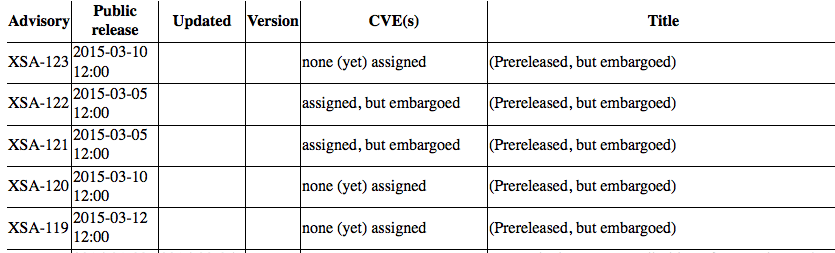
\includegraphics[scale=0.8]{pics/xsa.eps}
\end{center}
\vspace*{\fill}

\subsection{Current Events}
\verb+http://xenbits.xen.org/xsa/+ \\

\verb+https://aws.amazon.com/premiumsupport/maintenance-2015-03/+ \\

\verb+https://community.rackspace.com/general/f/53/t/4978+ \\

\verb+http://status.linode.com/incidents/2dyvn29ds5mz+


\subsection{Multiuser}

UNIX was designed from the beginning (1970s) as a portable, multi-tasking,
{\em multi-user} system. \\

Windows gained this functionality with WindowsNT in 1993. \\

Mac OS followed in 2001 with OS X.

\subsection{Implications of a Multi-User System}
\vspace*{\fill}
\begin{center}
	\includegraphics[scale=0.8]{pics/teamwork.eps}
\end{center}
\vspace*{\fill}

\subsection{Implications of a Multi-User System}
\vspace*{\fill}
\begin{center}
	
\includegraphics[scale=0.7]{pics/kids_fighting.eps}
\end{center}
\vspace*{\fill}

\subsection{Consider Scalability}
Things to consider:
\\

\begin{center}
	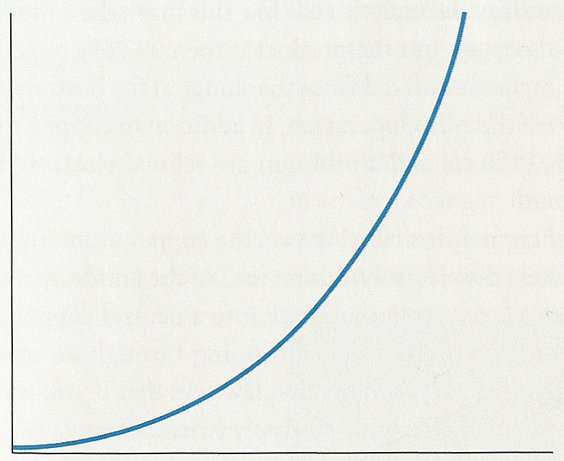
\includegraphics[scale=2.8]{pics/exponential_growth.eps}
\end{center}


\subsection{Granting Privileges requires Trust}
\begin{itemize}
	\item different environments have different trust models
	\item human interactions in small groups strengthen trust
	\item larger groups are divided into smaller, close-nit groups
	\item the more groups you have, the weaker their trust bonds are
\end{itemize}

\subsection{Granting Privileges requires Trust}
\begin{itemize}
	\item different environments have different trust models
	\item human interactions in small groups strengthen trust
	\item larger groups are divided into smaller, close-nit groups
	\item the more groups you have, the weaker their trust bonds are
\end{itemize}
\vspace{.5in}

\begin{center}
	\Huge
	{\bf Trust does not scale.}
	\Normalsize
\end{center}

\subsection{Granting Privileges requires Trust}
\vfill
\begin{center}
	\Huge
	Trust, but (be able to) verify.
	\Normalsize
\end{center}
\vfill

\subsection{Implications of a Multi-User System}
\vspace*{\fill}
\begin{center}
	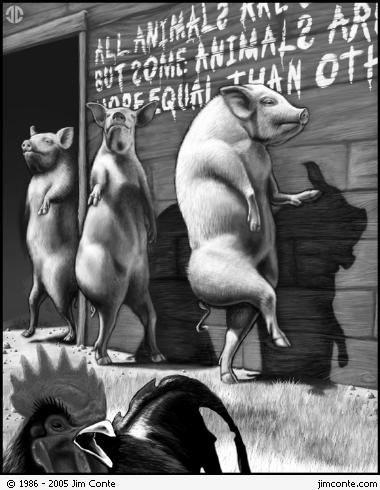
\includegraphics[scale=0.9]{pics/animal_farm.eps}
\end{center}
\vspace*{\fill}

\subsection{Implications of a Multi-User System}
\begin{itemize}
	\item users may want to keep files private
\end{itemize}

\subsection{Implications of a Multi-User System}
\begin{itemize}
	\item users may want to keep files private
	\item users may want to share files
\end{itemize}

\subsection{Implications of a Multi-User System}
\begin{itemize}
	\item users may want to keep files private
	\item users may want to share files
	\item users may (try to gain) access to files they shouldn't have access to
\end{itemize}

\subsection{Implications of a Multi-User System}
\begin{itemize}
	\item users may want to keep files private
	\item users may want to share files
	\item users may (try to gain) access to files they shouldn't have access to
	\item users may (want to) do things that affect other users
\end{itemize}

\subsection{Implications of a Multi-User System}
\begin{itemize}
	\item users may want to keep files private
	\item users may want to share files
	\item users may (try to gain) access to files they shouldn't have access to
	\item users may (want to) do things that affect other users
	\item different users may require different privileges
\end{itemize}

\subsection{Users and User-IDs}
\begin{center}
	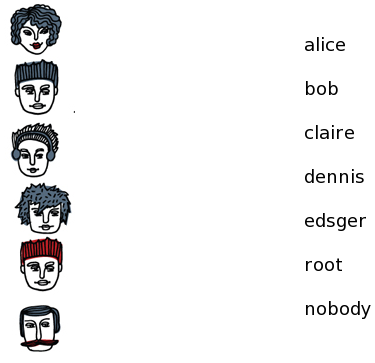
\includegraphics[scale=0.9]{pics/user-sets0.eps} \\
	Bijective?
\end{center}

\subsection{Users and User-IDs}
\begin{center}
	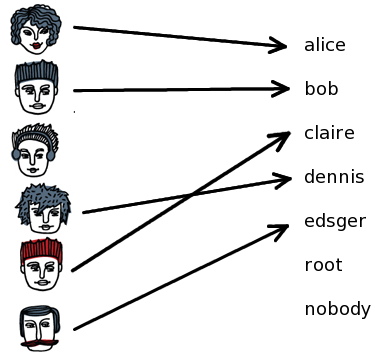
\includegraphics[scale=0.9]{pics/user-sets1.eps} \\
	{\em Not} surjective!
\end{center}

\subsection{Users and User-IDs}
\begin{center}
	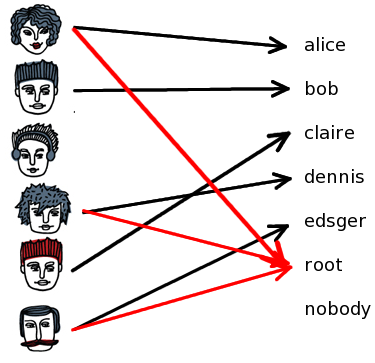
\includegraphics[scale=0.9]{pics/user-sets2.eps} \\
	{\em Not} injective, either!
\end{center}

\subsection{Users and User-IDs}

\begin{center}
	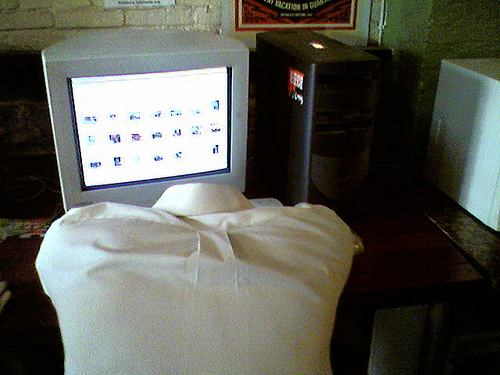
\includegraphics[scale=0.8]{pics/headless.eps} \\
	{\tt nobody}
\end{center}

\subsection{UNIX Fundamentals: User Accounts and File Permissions}
Every account
\begin{itemize}
	\item has a {\em unique} ID
	\item belongs to at least one group
	\item may or may not be password protected
	\item may or may not have a valid login program
	\item may or may not be allowed to escalate privileges
\end{itemize}

\subsection{UNIX Fundamentals: User Accounts and File Permissions}
Every account
\begin{itemize}
	\item has a {\em unique} ID
	\item belongs to at least one group
	\item may or may not be password protected
	\item may or may not have a valid login program
	\item may or may not be allowed to escalate privileges
\end{itemize}
\addvspace{.5in}
Every file
\begin{itemize}
	\item is associated with a {\em uid} and a {\em gid}
	\item has a number of protection bits
\end{itemize}

\subsection{UNIX Fundamentals: User Accounts and File Permissions}
\vfill
\begin{center}
	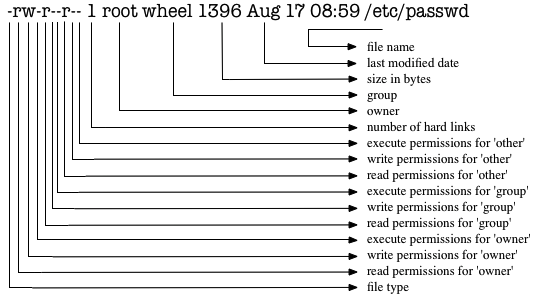
\includegraphics[scale=0.9]{pics/ls-l.eps}
\end{center}
\vfill

\subsection{Unix Groups}
\begin{itemize}
	\item enables {\em arbitrary} collections of users to share resources
	\item information stored in \verb+/etc/group+, format is: \\
		\verb+name:*:GID:user1,user2,...+
	\item most Unix systems impose a limit of 16 or 32 group memberships per
		user
	\item most Unix systems have a common default group for new users (some
		Linux versions deviate)
	\item some Unix systems have group shadow files
\end{itemize}

\subsection{Group Access}
At any but the smallest environments, we find:
\begin{itemize}
	\item a central user database
	\item users divided into different access groups
	\item access to systems is granted primarily by such group membership
	\item privileges on a system are also granted by such group membership
\end{itemize}

\subsection{Group Access}
\begin{center}
	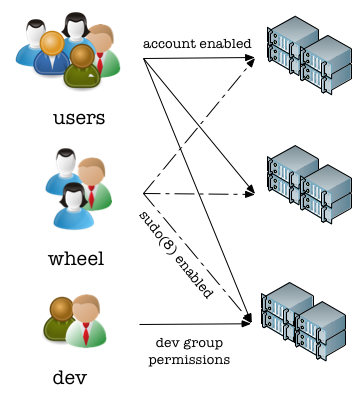
\includegraphics[scale=0.8]{pics/groups-machines.eps}
\end{center}

\subsection{Adding and Removing Accounts}

\vfill
In-class exercise: \\
\verb+https://www.cs.stevens.edu/~jschauma/615/useradd-exercise.html+
\vfill

\subsection{Adding and Removing Accounts}
\vfill
In-class exercise: \\
\verb+https://www.cs.stevens.edu/~jschauma/615/useradd-exercise.html+

\vspace{.5in}
Accounts management is done centrally; changes are applied to machines via a
configuration management system and/or directory service.
\vfill

\subsection{Ethics}
\begin{center}
	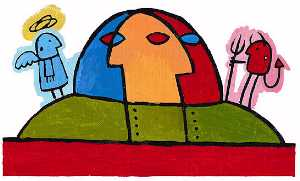
\includegraphics[scale=2.5]{pics/angel-devil.eps}
\end{center}

\subsection{You are a Super User!}
\begin{center}
	
\includegraphics[scale=1.0]{pics/superman.eps} \\
	\small
	Yes, you are!
	\Normalsize
\end{center}

\subsection{You are a Super User!}
\begin{center}
	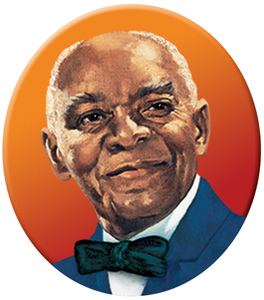
\includegraphics[scale=4.0]{pics/uncle-ben.eps} \\
	\addvspace{.2in}
	\Huge
	``With great power comes great responsibility.''
	\Normalsize
\end{center}

\subsection{sudo(8)}
\vspace*{\fill}
\begin{verbatim}
We trust you have received the usual lecture from the local System
Administrator. It usually boils down to these three things:
#1) Respect the privacy of others.
#2) Think before you type.
#3) With great power comes great responsibility.
\end{verbatim}
\vspace*{\fill}

\subsection{Ethics}
The LISA Code of Ethics:
\\

\newcolumntype{S}{>{\centering\arraybackslash} m{.4\linewidth} }
\begin{tabular}{ p{10cm} S }
\begin{itemize}
	\item Professionalism
	\item Personal Integrity
	\item Privacy
	\item Laws and Policies
	\item System Integrity
	\item Education
	\item Social Responsibility
	\item Ethical Responsibility
\end{itemize}
& \multirow{20}{*}{
\includegraphics[scale=1.3]{pics/angel.eps}} \\
\end{tabular}

\subsection{Ethics: This stuff isn't easy!}
\begin{center}
	
\includegraphics[scale=0.3]{pics/snowden.eps}
\end{center}

\subsection{Ethics: Professionalism}
\vfill
\begin{center}
I will maintain professional conduct in the workplace and will not allow
personal feelings or beliefs to cause me to treat people unfairly or
unprofessionally.
\end{center}
\vfill

\subsection{Ethics: Personal Integrity}
\vfill
\begin{center}
I will be honest in my professional dealings and forthcoming about my
competence and the impact of my mistakes. I will seek assistance from
others when required. \\
\vspace{.5in}

I will avoid conflicts of interest and biases whenever possible. When my
advice is sought, if I have a conflict of interest or bias, I will declare
it if appropriate, and recuse myself if necessary.
\end{center}
\vfill


\subsection{Ethics: Privacy}
\vfill
\begin{center}
I will access private information on computer systems only when it is
necessary in the course of my technical duties. I will maintain and
protect the confidentiality of any information to which I may have access,
regardless of the method by which I came into knowledge of it.
\end{center}
\vfill

\subsection{Ethics: Laws and Policies}
\vfill
\begin{center}
I will educate myself and others on relevant laws, regulations, and
policies regarding the performance of my duties.
\end{center}
\vfill

\subsection{Ethics: Communication}
\vfill
\begin{center}
I will communicate with management, users, and colleagues about computer
matters of mutual interest. I will strive to listen to and understand the
needs of all parties.
\end{center}
\vfill

\subsection{Ethics: System Integrity}
\vfill
\begin{center}
I will strive to ensure the necessary integrity, reliability, and
availability of the systems for which I am responsible. \\
\vspace{.5in}

I will design and maintain each system in a manner to support the
purpose of the system to the organization.
\end{center}
\vfill

\subsection{Ethics: Education}
\vfill
\begin{center}
I will continue to update and enhance my technical knowledge and other
work-related skills. I will share my knowledge and experience with others.
\end{center}
\vfill

\subsection{Ethics: Responsibility to the Computing Community}
\vfill
\begin{center}
I will cooperate with the larger computing community to maintain the
integrity of network and computing resources.
\end{center}
\vfill

\subsection{Ethics: Social Responsibility}
\vfill
\begin{center}
As an informed professional, I will encourage the writing and adoption of
relevant policies and laws consistent with these ethical principles.
\end{center}
\vfill

\subsection{Ethics: Ethical Responsibility}
\vfill
\begin{center}
I will strive to build and maintain a safe, healthy, and productive
workplace. \\
\vspace{.5in}

I will do my best to make decisions consistent with the safety, privacy,
and well-being of my community and the public, and to disclose promptly
factors that might pose unexamined risks or dangers. \\
\vspace{.5in}

I will accept and offer honest criticism of technical work as appropriate
and will credit properly the contributions of others. \\
\vspace{.5in}

I will lead by example, maintaining a high ethical standard and degree
of professionalism in the performance of all my duties. I will support
colleagues and co-workers in following this code of ethics.

\end{center}
\vfill

\subsection{At the end of the day...}
\begin{center}
	
\includegraphics[scale=0.5]{pics/thumbsup-borat.eps}
\end{center}


\newpage
\vspace*{\fill}
\begin{center}
    \Hugesize
        Hooray! \\ [1em]
    \hspace*{5mm}
    \blueline\\
    \hspace*{5mm}\\
        5 Minute Break
\end{center}
\vspace*{\fill}

\newpage
\vspace*{\fill}
\begin{center}
	\Hugesize
		Automation and Scripting \\ [1em]
	\hspace*{5mm}
	\blueline\\
	\hspace*{5mm}\\
		Part I
\end{center}
\vspace*{\fill}

\subsection{What should be automated?}

\begin{itemize}
	\item software installation / upgrades / audits
	\item account creation / deletion
	\item system configuration changes
	\item log and event processing
\end{itemize}
\vspace{.5in}
...and anything / everything else in between!

\subsection{Words of Wisdom}
\\

\newcommand{\gargantuan}{\fontsize{60}{65}\selectfont}
\gargantuan
\begin{center}
Anything you do more than once is worth automating.
\end{center}
\Normalsize



\subsection{Why automate anything?}

\subsection{Why automate anything?}
\begin{itemize}
	\item we're lazy
\end{itemize}

\subsection{Why automate anything?}
\begin{itemize}
	\item we're lazy
	\item we're unreliable and make mistakes
\end{itemize}

\subsection{Why automate anything?}
\begin{itemize}
	\item we're lazy
	\item we're unreliable and make mistakes
	\item we're forgetful
\end{itemize}

\subsection{Who do we automate things for?}
\subsection{Who do we automate things for?}
\begin{itemize}
	\item ourselves
\end{itemize}

\subsection{Who do we automate things for?}
\begin{itemize}
	\item ourselves
	\item our peers
\end{itemize}

\subsection{Who do we automate things for?}
\begin{itemize}
	\item ourselves
	\item our peers
	\item our users
\end{itemize}

\subsection{Who do we automate things for?}
\begin{itemize}
	\item ourselves
	\item our peers
	\item our users
	\item anybody else
\end{itemize}

\subsection{Tools}
\vspace*{\fill}
\begin{center}
	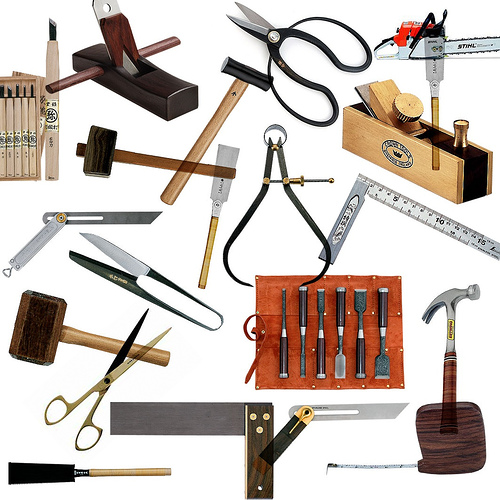
\includegraphics[scale=1.4]{pics/tools.eps}
\end{center}
\vspace*{\fill}

\subsection{The right tool?}
\vspace*{\fill}
\begin{center}
	
\includegraphics[scale=0.6]{pics/hammer.eps}
\end{center}
\vspace*{\fill}

\subsection{The right tool?}
\vspace*{\fill}
\begin{center}
	
\includegraphics[scale=2.5]{pics/nails.eps}
\end{center}
\vspace*{\fill}

\subsection{The right tool?}
\vspace*{\fill}
\begin{center}
	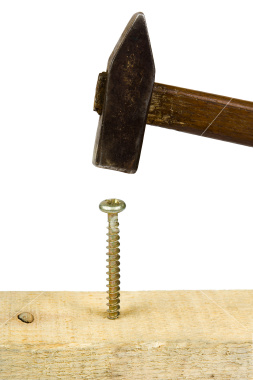
\includegraphics[scale=3]{pics/hammer-screw.eps}
\end{center}
\vspace*{\fill}

\subsection{The right tool?}
Bourne shell (/bin/sh) \\

\begin{itemize}
	\item lowest common denominator
	\item available and reliable on most platforms (but beware of non-portable
		bash(1) "enhancements")
	\item beware of "quick-and-dirty" solutions, they grow to become
		unmaintainable
	\item treat shell as any other programming language:
		\begin{itemize}
			\item use functions
			\item use suitably scoped variables
			\item follow Unix philosophy
			\item properly package your tool
		\end{itemize}
\end{itemize}


\subsection{The right tool?}
Perl, Python, Ruby, ... \\

\begin{itemize}
	\item suitable for moderately complex tasks
	\item move to these when sed(1), awk(1), etc. become too cumbersome
	\item text manipulation frequently easier
	\item beware of "quick-and-dirty" solutions, they grow to become
		unmaintainable
	\item try to build self-contained modules that can be tested independent of
		the "main" program
	\item wealth of libraries available -- use them! (And remember to explicitly
		require them.)
	\item properly package your tool
\end{itemize}

\subsection{The right tool?}
Perl, PHP, Tcl, JavaScript, CoffeeScript, ... \\

\begin{itemize}
	\item http/web server interfaces
	\item CGI "scripts" / server-side execution (e.g. NodeJS)
	\item interface with/utilize APIs in a specific domain/vendor products
	\item frequent cause of all sorts of security problems due to interface with
		user data / exposure on the internet
\end{itemize}

\subsection{The right tool?}
Java, Scala, Clojure, Rhino, ... \\

\begin{itemize}
	\item know your primary applications
	\item interface with / extend / tie into JVM
\end{itemize}

\subsection{The right tool?}
C, C++, Go, Rust, ... \\

\begin{itemize}
	\item performance benefits
	\item portability
	\item sufficient low-levelness
	\item systems understanding
	\item fix/patch your other tools / the system
\end{itemize}

\subsection{Interpreted Languages}
General advantages: \\

\begin{itemize}
	\item short development cycle
	\item normally facilitate things like string manipulation, arithmetic and
		more complex regular expressions
	\item easily handle multiple file handles and other I/O
	\item some security features
	\item tens of thousands of special- and general-purpose modules available
\end{itemize}

\subsection{Interpreted Languages}
General Disadvantages: \\

\begin{itemize}
	\item no one tool fits all purposes
	\item tens of thousands of special- and general-purpose modules available $=>$
		lots of duplication, stale code, questionable quality
	\item security features frequently neglected or circumvented ("too hard" or
		more precisely "inconvenient")
	\item everybody has their particular favorite (and dislikes one or the
		other)
	\item interpreter not (necessarily) universally available / installed
\end{itemize}

\subsection{Approaching Automation}
Three basic categories:
\\

\begin{itemize}
	\item scripting
	\item programming
	\item software engineering
\end{itemize}

\subsection{Approaching Automation}
Three basic categories:
\\
\begin{itemize}
	\item scripting
\end{itemize}
\vspace*{\fill}
\begin{center}
	
\includegraphics[scale=0.5]{pics/hammer.eps}
\end{center}
\vspace*{\fill}


\subsection{Approaching Automation}
Three basic categories:
\\

\begin{itemize}
	\item scripting
		\begin{itemize}
			\item automating {\em very} simple tasks
		\end{itemize}
\end{itemize}

\subsection{Approaching Automation}
Three basic categories:
\\

\begin{itemize}
	\item scripting
		\begin{itemize}
			\item automating {\em very} simple tasks
			\item customization of user environment
		\end{itemize}
\end{itemize}

\subsection{Approaching Automation}
Three basic categories:
\\

\begin{itemize}
	\item scripting
		\begin{itemize}
			\item automating {\em very} simple tasks
			\item customization of user environment
			\item often only suitable for one individual user
		\end{itemize}
\end{itemize}

\subsection{Approaching Automation}
Three basic categories:
\\

\begin{itemize}
	\item scripting
		\begin{itemize}
			\item automating {\em very} simple tasks
			\item customization of user environment
			\item often only suitable for one individual user
			\item usually eventually evolves into larger programs
		\end{itemize}
\end{itemize}

\subsection{Approaching Automation}
Three basic categories:
\\

\begin{itemize}
	\item programming
\end{itemize}
\vspace*{\fill}
\begin{center}
	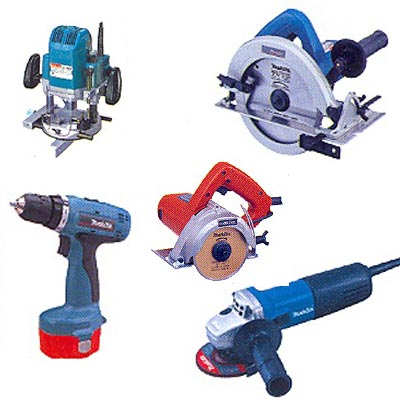
\includegraphics[scale=0.8]{pics/power-tools.eps}
\end{center}
\vspace*{\fill}



\subsection{Approaching Automation}
Three basic categories:
\\

\begin{itemize}
	\item programming
		\begin{itemize}
			\item suitable for simple to moderately complex tasks
		\end{itemize}
\end{itemize}

\subsection{Approaching Automation}
Three basic categories:
\\

\begin{itemize}
	\item programming
		\begin{itemize}
			\item suitable for simple to moderately complex tasks
			\item results frequently used by a small base of users
		\end{itemize}
\end{itemize}

\subsection{Approaching Automation}
Three basic categories:
\\

\begin{itemize}
	\item programming
		\begin{itemize}
			\item suitable for simple to moderately complex tasks
			\item results frequently used by a small base of users
			\item uses basic framework or common toolkits
		\end{itemize}
\end{itemize}

\subsection{Approaching Automation}
Three basic categories:
\\

\begin{itemize}
	\item programming
		\begin{itemize}
			\item suitable for simple to moderately complex tasks
			\item results frequently used by a small base of users
			\item uses basic framework or common toolkits
			\item provides consistent interface
		\end{itemize}
\end{itemize}

\subsection{Approaching Automation}
Three basic categories:
\\

\begin{itemize}
	\item programming
		\begin{itemize}
			\item suitable for simple to moderately complex tasks
			\item results frequently used by a small base of users
			\item uses basic framework or common toolkits
			\item provides consistent interface
			\item may evolve into full product
		\end{itemize}
\end{itemize}

\subsection{Approaching Automation}
Three basic categories:
\\

\begin{itemize}
	\item software development
\end{itemize}
\vspace*{\fill}
\begin{center}
	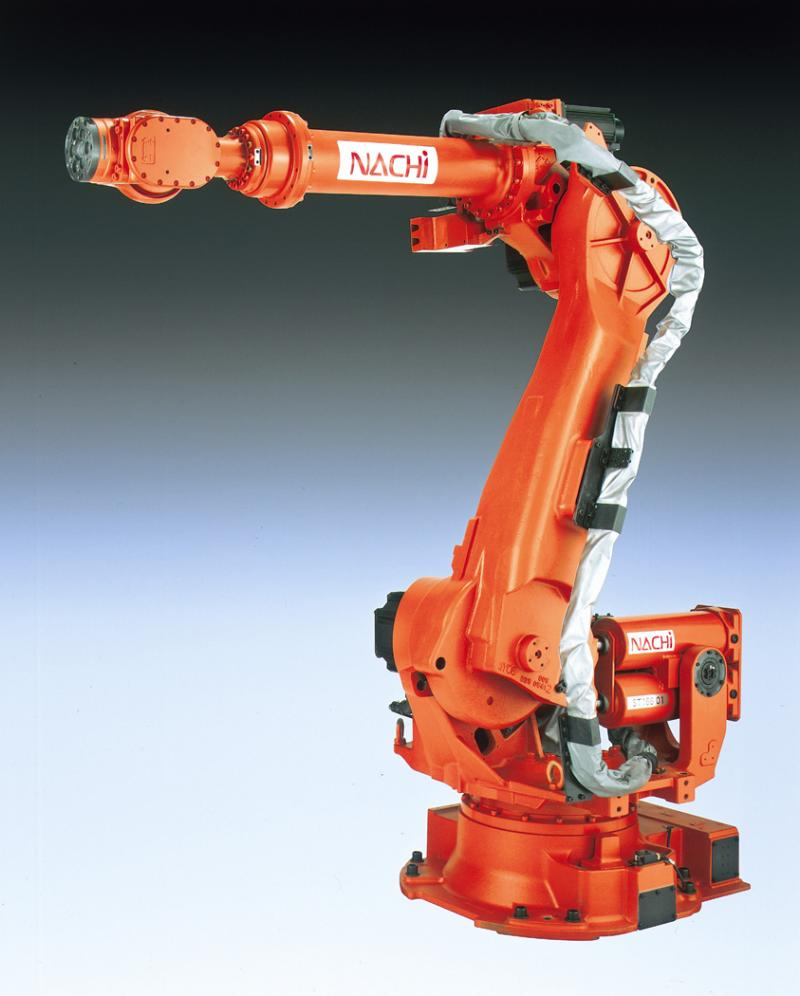
\includegraphics[scale=0.25]{pics/big-tool.eps}
\end{center}
\vspace*{\fill}


\subsection{Approaching Automation}
Three basic categories:
\\

\begin{itemize}
	\item software development
		\begin{itemize}
			\item required for any reasonably complex task
		\end{itemize}
\end{itemize}

\subsection{Approaching Automation}
Three basic categories:
\\

\begin{itemize}
	\item software development
		\begin{itemize}
			\item required for any reasonably complex task
			\item uses formal software engineering approach (measurable goals,
				requirements, specifications, ...)
		\end{itemize}
\end{itemize}

\subsection{Approaching Automation}
Three basic categories:
\\

\begin{itemize}
	\item software development
		\begin{itemize}
			\item required for any reasonably complex task
			\item uses formal software engineering approach (measurable goals,
				requirements, specifications, ...)
			\item may evolve from previous prototypes
		\end{itemize}
\end{itemize}


\subsection{Approaching Automation}
Three basic categories:
\\

\begin{itemize}
	\item software development
		\begin{itemize}
			\item required for any reasonably complex task
			\item uses formal software engineering approach (measurable goals,
				requirements, specifications, ...)
			\item may evolve from previous prototypes
			\item requires ongoing continous maintenance / development efforts
		\end{itemize}
\end{itemize}

\subsection{Where are you?}
Make sure to understand your requirements:

\begin{itemize}
	\item motivation / goals
	\item target audience
	\item scope
	\item dependencies
\end{itemize}

\subsection{Reading}
User Management:
\begin{itemize}
	\item {\em Frisch}: Ch 6; {\em Burgess}: Ch 5;
\end{itemize}
\vspace{.5in}
\begin{itemize}
	\item http://nixsrv.com/llthw/ex23
\end{itemize}
\vspace{.5in}
Ethics:
\begin{itemize}
	\item \verb+https://www.usenix.org/lisa/system-administrators-code-ethics+
	\item \verb+http://www.acm.org/about/code-of-ethics+
\end{itemize}

\subsection{Professional Organizations}
\begin{itemize}
	\item \verb+https://www.usenix.org/+ and \verb+https://www.usenix.org/lisa+
	\item \verb+http://www.lopsa.org/+
	\item \verb+http://www.acm.org/+
	\item \verb+https://www.internetsociety.org/+
	\item \verb+https://www.nanog.org/+
\end{itemize}

\subsection{Reading}
Shell:
\begin{itemize}
	\item \verb+http://www.tldp.org/HOWTO/Bash-Prog-Intro-HOWTO.html+
	\item \verb+http://www.tldp.org/LDP/abs/html/+
	\item \verb+http://sed.sourceforge.net/sed1line.txt+
	\item \verb+csh(1)+, \verb+ksh(1)+, \verb+sh(1)+
	\item {\em Frisch}: Chapter 3, 14
\end{itemize}
%
\end{document}
